\chapter{The smoothness assumption in the global algorithm}
The last part of our work focuses on the addition of the smoothness constraint to the overall algorithm described in chapter \ref{sec:GD}.
\section{Results}
Again, the starting conditions for the experiments are analogues to the ones supposed in chapters \ref{sec:GD} and \ref{sec:DL}, the number of iterations is, again, $250$ and there is still a rate $5:1$ for the number of iterations dedicated to the graph learning part, per each iteration dedicated to the dictionary learning one.
\\

The figures \ref{fig:alphaHeatGD_smth} and \ref{fig:alphaDorinaGD_smth} show the comparison between the kernels learned without and with the smoothness assumption. In both the figures we see how the smoothness assumption still improves the kernel learning process, at the same time respecting the overall spectral composition of the signal.

\begin{figure}
  \centering
  \begin{minipage}[c]{.8\textwidth}
    \centering
    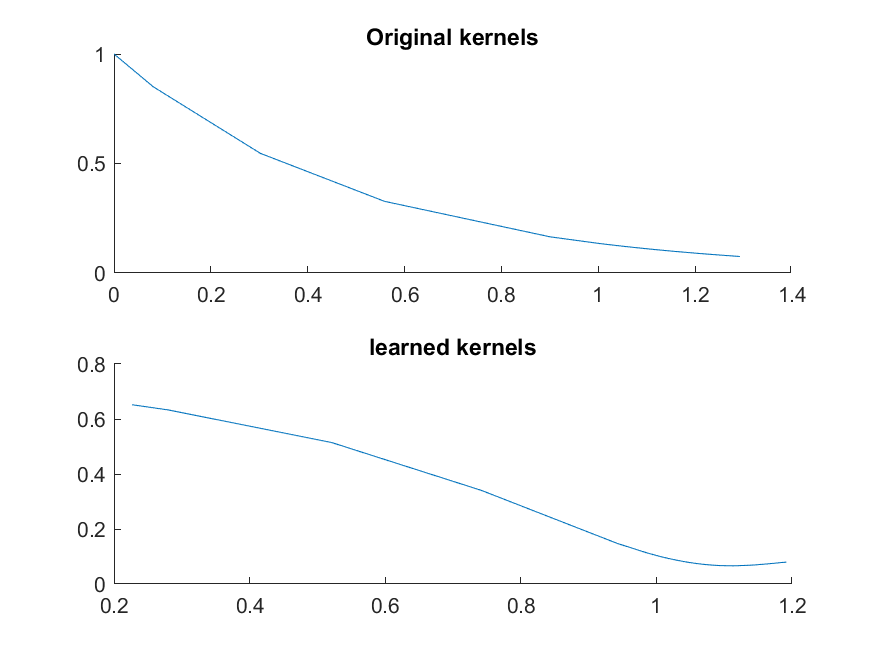
\includegraphics[width = \textwidth]{kernelHeat_noSmoothness_GD.png}
  \end{minipage}
  \begin{minipage}[c]{.8\textwidth}
    \centering
    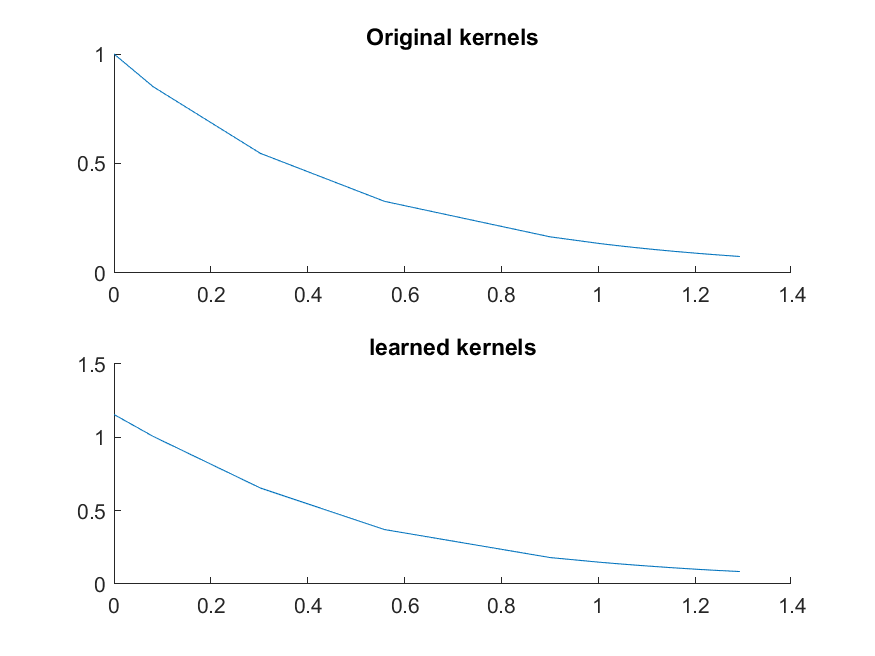
\includegraphics[width = \textwidth]{kernelHeat_Smoothness_struct.png}
  \end{minipage}
  \caption{Comparison between kernels coefficients without and with smoothness prior. Heat kernel dataset}
  \label{fig:alphaHeatGD_smth}
\end{figure}

\begin{figure}
  \centering
  \begin{minipage}[c]{.8\textwidth}
    \centering
    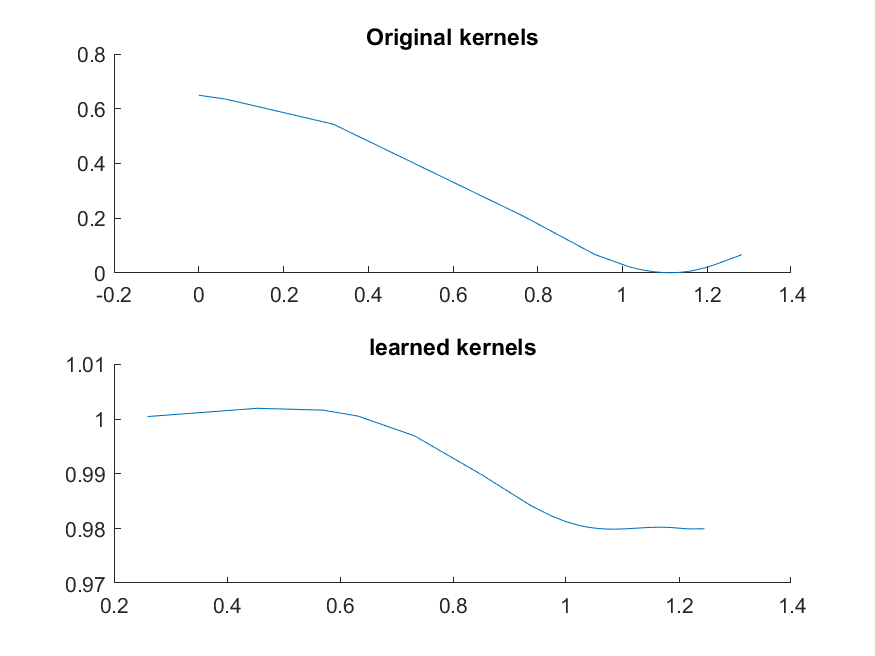
\includegraphics[width = \textwidth]{kernelDorina_GD.png}
  \end{minipage}
  \begin{minipage}[c]{.8\textwidth}
    \centering
    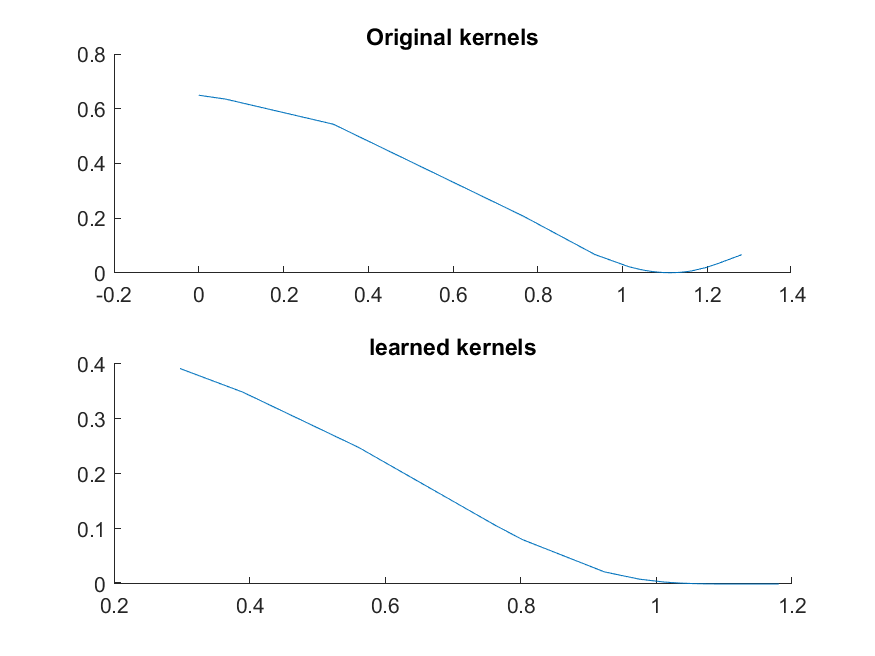
\includegraphics[width = \textwidth]{kernelDorina_Smoothness_GD_struct.png}
  \end{minipage}
  \caption{Comparison between kernels coefficients without and with smoothness prior. Thanou et al. dataset}
  \label{fig:alphaDorinaGD_smth}
\end{figure}

Table \ref{tab:PrecRec_compSmth} again shows the comparison between the Precision and Recall values obtained from the approach without the smoothness prior and the approach accounting for it. The values listed clearly show how, in the case of the Thanou kernel, the algorithm benefits from the prior, having both the values increased. For what concerns the second dataset the results tend to worsen, even though better values are sometimes achieved.

\begin{table}[htbp]
  \centering
  \begin{tabular}{lcccc}
  &\multicolumn{2}{c}{\textbf{Heat kernel}}&\multicolumn{2}{c}{\textbf{Thanou et al. kernel}}\\
  \toprule
  &No Smoothness & Smoothness & No Smoothness & Smoothness\\ %\cline{2-5}
    \midrule
    \textbf{Precision rate} & 91.97 \% & 76.48 \% & 69.277 \% & 86.05 \%\\
    \textbf{Recall Rate} & 91.66 \% & 76.48 \% & 67.69 \% & 84.66 \%\\
    \bottomrule
  \end{tabular}
  \caption{Precision and Recall outputs for the low frequency kernel from Thanou et al. dataset}
  \label{tab:PrecRec_compSmth}
\end{table}

Having a look in detail, now, to the reproduction error, we can observe how in this general case the algorithm tends to behave better for the Thanou et al. dataset, while it's almost the same for the heat kernel dataset. \autoref{tab:errorGD_smoothness} compares the reproduction error over $3$ trials for both the datasets, and shows how not only the smoothness prior improves the outcomes, but the algorithm results in being more stable over the trials.

\begin{table}[htbp]
  \centering
  \begin{tabular}{lcccc}
  \textbf{Trial \#} &\multicolumn{2}{c}{\textbf{Heat kernel}}&\multicolumn{2}{c}{\textbf{Thanou et al. kernel}}\\
  \toprule
  & No Smoothness & Smoothness & No Smoothness & Smoothness\\ %\cline{2-5}
  \midrule
    1 & 0.1114 & 0.1113 & 0.0225 & 0.0230\\
    2 & 0.0310 & 0.1131 & 0.0384 & 0.0229\\
    3 & 0.1024 & 0.1100 & 0.0239 & 0.0224\\
    \textbf{Average Error} & 0.0816 & 0.1115 & 0.0283 & 0.0227 \\
    \bottomrule
  \end{tabular}
  \caption{Reproduction error comparison for the low frequency kernel from both the datasets}
  \label{tab:errorGD_smoothness}
\end{table}

Moreover, for what concerns the kernels coefficients, figures \ref{fig:alphaGDHeat} and \ref{fig:alphaGDDorina} highlight one time more how the smoothness prior has a good repercussion over them, allowing to get more faithful behaviors.

\begin{figure}
  \centering
  \begin{minipage}[c]{.8\textwidth}
    \centering
    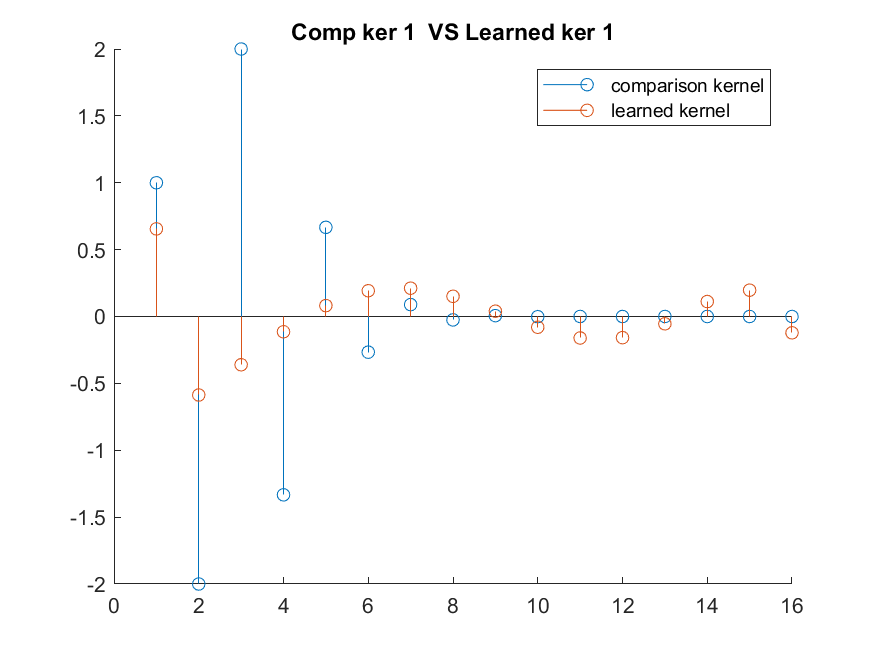
\includegraphics[width = \textwidth]{alphaHeat_noSmoothness_GD.png}
  \end{minipage}
  \begin{minipage}[c]{.8\textwidth}
    \centering
    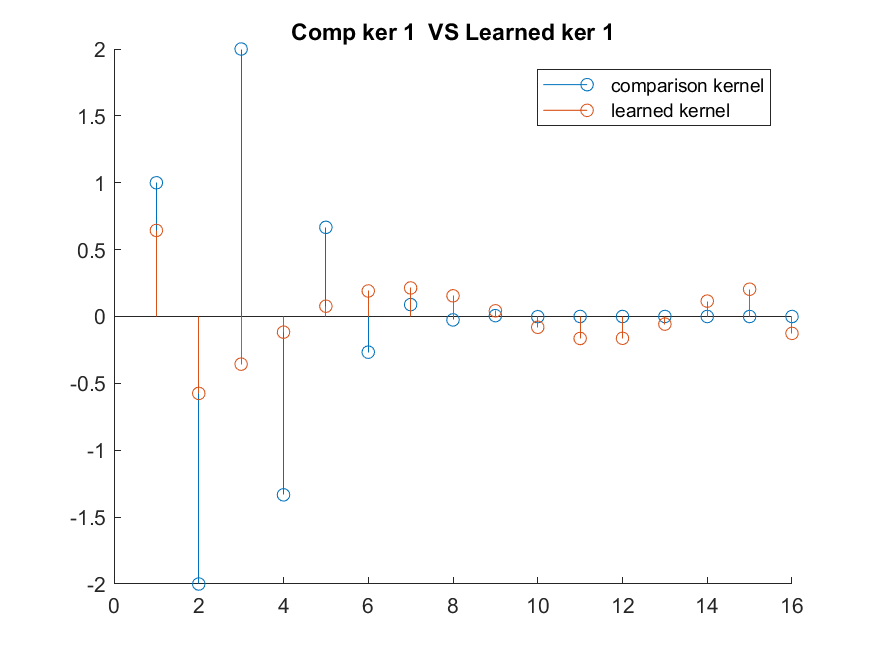
\includegraphics[width = \textwidth]{alphaHeat_Smoothness_GD_struct.png}
  \end{minipage}
  \caption{Comparison between kernels coefficients without and with smoothness prior. Heat kernel   dataset}
  \label{fig:alphaGDHeat}
\end{figure}

\begin{figure}
  \centering
  \begin{minipage}[c]{.8\textwidth}
    \centering
    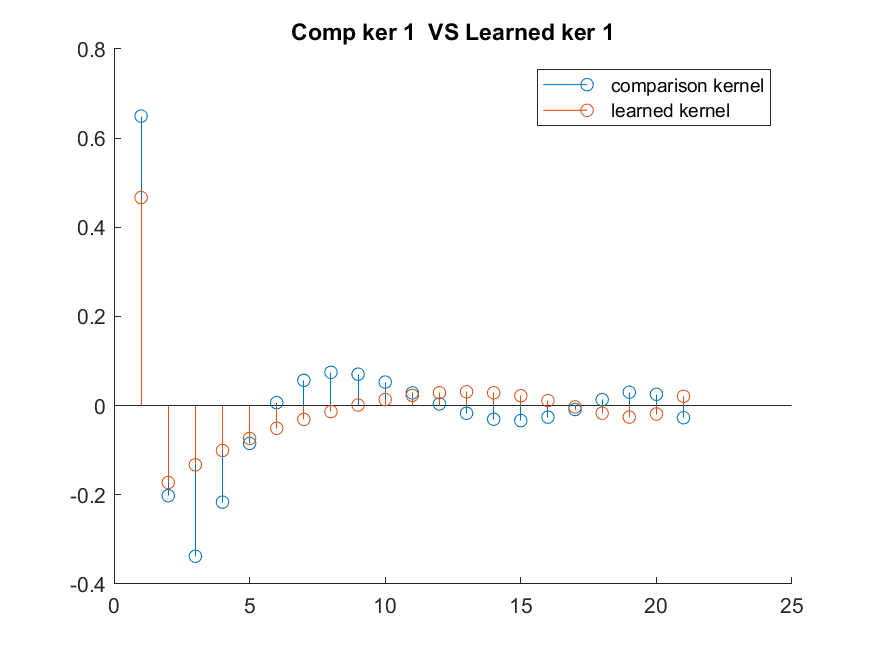
\includegraphics[width = \textwidth]{alphaDorina_noSmoothness_GD.png}
  \end{minipage}
  \begin{minipage}[c]{.8\textwidth}
    \centering
    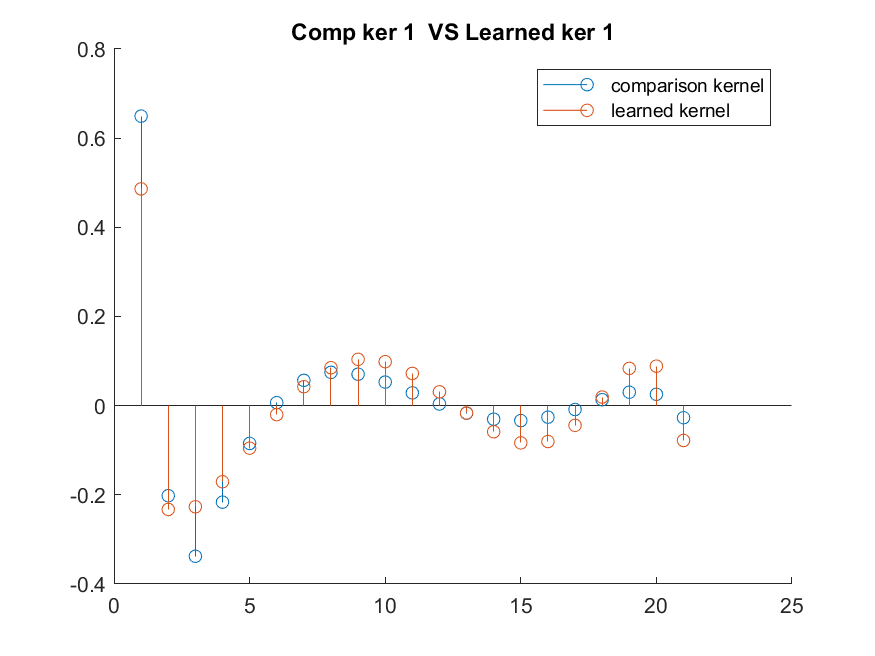
\includegraphics[width = \textwidth]{alphaDorina_Smoothness_GD_struct.png}
  \end{minipage}
  \caption{Comparison between kernels coefficients without and with smoothness prior. Thanou et al.   dataset}
  \label{fig:alphaGDDorina}
\end{figure}

Finally, in we examine the computational cost of the algorithm with and without the prior, we can see a general improvement of the average CPUTime per iteration, as shown in \autoref{tab:CPUTime_GD}

\begin{table}[htbp]
  \centering
  \begin{tabular}{lcccc}
  \textbf{Trial \#} &\multicolumn{2}{c}{\textbf{Heat kernel}}&\multicolumn{2}{c}{\textbf{Thanou et al. kernel}}\\
  \toprule
  & No Smoothness & Smoothness & No Smoothness & Smoothness\\ %\cline{2-5}
  \midrule
    1 & 0.0219 & 0.0164 & 0.0267 & 0.0128\\
    2 & 0.0163 & 0.0171 & 0.0253 & 0.0123\\
    3 & 0.0328 & 0.0166 & 0.0269 & 0.0155\\
    \textbf{Average CPUTime} & 0.0191 & 0.0167 & 0.0263 & 0.0135 \\
    \bottomrule
  \end{tabular}
  \caption{Computational cost comparison for both the datasets with an without smoothness priors}
  \label{tab:CPUTime_GD}
\end{table}
